\chapter{Beispielhafte Anwendung der erarbeiteten Methoden}
\section{Das Spiel}
Dieser Abschnitt soll einen grundlegenden Überblick über das Spiel gewähren, für welches die modularen Gebäude erstellt werden.
\begin{description}
\item[Grundlagen]~\par
Bei \textit{Renegade Line} handelt es sich um einen Third Person Cartoon Shooter, in dem bis zu 16 Spieler über das Internet in verschiedenen Spielmodi auf unterschiedlichen Karten gegeneinander spielen können. In den meisten Spielmodi werden die Spieler in zwei Teams mit jeweils acht Spielern eingeteilt, die im Anschluss um den Sieg kämpfen. Spieler können während des Spiels eine von vier verschiedenen Klassen wählen, die spezielle Fähigkeiten und passende Waffen besitzen.
\par
Das Spiel befindet sich zum Zeitpunkt dieser Thesis im Early Access und wird von Raw Vengeance Studios entwickelt. Raw Vengeance ist ein kleines Start-up aus Hamburg. Aktuell wird eine neue Karte für einen neuen Spielmodus entwickelt. Zusammen mit der neuen Karte soll auch ein neues Setting etabliert werden. Bisher wurden alle Modelle für die neue Karte von mir erstellt.
\item[Der Stil]~\par
Der Stil des Spieles ist ein stilisierter Cartoon Look. Alle Elemente sind Abwandlungen ihrer realen Gegenstücke. Meist werden prägnante Formen stark hervorgehoben. Das bisherige Setting aller Assets ist leicht stereotypisierend an eine italienische Kleinstadt angelehnt (vgl. Abbildung \ref{altSetting}). Das neue Setting soll das feudale Japan repräsentieren. Auch hier wird mit Stereotypen gearbeitet, die eindeutig und leicht zu erkennen sein sollen. In \textit{Renegade Line} können Gebäude nicht betreten werden, alle Handlungen finden im Freien stattfinden. Dies reduziert die Komplexität der Modelle und die Arbeitszeit ihrer Erstellung.
\end{description}
\begin{figure}[!h]
\centering
  \makebox[\textwidth]{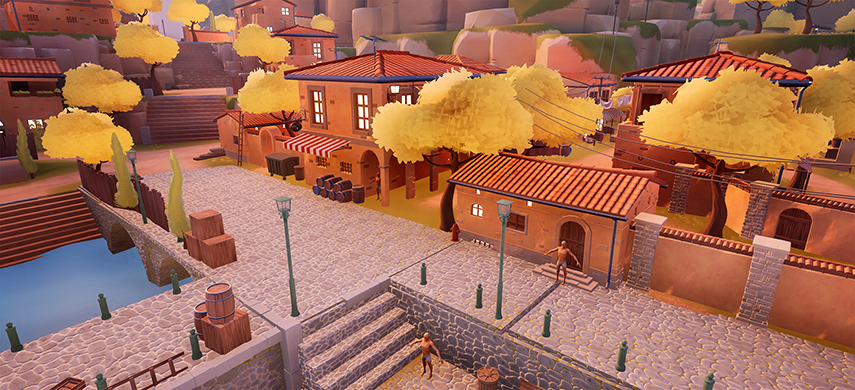
\includegraphics[width=0.94\linewidth]{bilder/altSetting}}
  \caption{Ausschnitt eines aktuellen Levels in dem bisherigen Setting.}
	\label{altSetting}
\end{figure}
\section{Durchführung}
Die folgenden Abschnitte behandeln die Anwendung der zuvor erarbeiteten Methoden.
\subsection{Planung}
In der Planungsphase wurde in Zusammenarbeit mit dem Lead-Level-Designer definiert, welche Anforderungen das Kit erfüllen soll. Es wurde über den generellen Aufbau der Gebäude gesprochen. Dies umfasst die Größe der Grundrisse, die Anzahl der Stockwerke, welche Elemente eine Etage ausmachen sollen und welche Sonder-Elemente es geben soll. Außerdem wurde das Design der verschiedenen Elemente angesprochen. Die Umsetzung der Anforderungen habe ich selbst ausgearbeitet.
\par
Diese Anforderungen wurden festgelegt:
\begin{description}
\item[Grundriss]\hfill
\begin{itemize}[leftmargin=0cm]
\item Gebäude sollen nicht nur rechteckig, sondern auch in anderen Formen aufgebaut sein (L-Form, Kreuz etc..) und
\item die Grundfläche eines Gebäudes soll nach Möglichkeit unlimitiert sein.
\end{itemize}
\item[Etagen]\hfill
\begin{itemize}[leftmargin=0cm]
\item Es sollen mindestens fünf oder besser unbegrenzt viele Etagen möglich sein und
\item in der untersten Etage soll ein Steinfundament mit einer Treppe einzusetzen eingesetzt werden können.
\end{itemize}
\item[Details]\hfill
\begin{itemize}[leftmargin=0cm]
\item Es soll Elemente für ein Vordach geben, das eine Art Umrandung um das Gebäude bildet (Abbildung \ref{KitelementeSkizze} auf Seite \pageref{KitelementeSkizze} ),
\item Wandstücke sollen in verschiedenen Ausführungen erstellt werden: mit unterschiedlichen Holzmustern, Fenstern und Türen und
\item es soll Elemente für einen Balkon geben, wenn möglich.
\end{itemize}
\item[Design]\hfill
\begin{itemize}[leftmargin=0cm]
\item Die Farbgebung soll sich an Abbildung \ref{JapanKonzept} (Folgeseite) und dem bisherigen Farbspektrum orientieren und
\item das grundlegende Design der Gebäude soll sich an Abbbildung \ref{JapanKonzept} (Folgeseite) und Abbildung \ref{KitelementeSkizze} (Seite \pageref{KitelementeSkizze}) orientieren.
\end{itemize}
\end{description}
\begin{figure}[!h]
\centering
  \makebox[\textwidth]{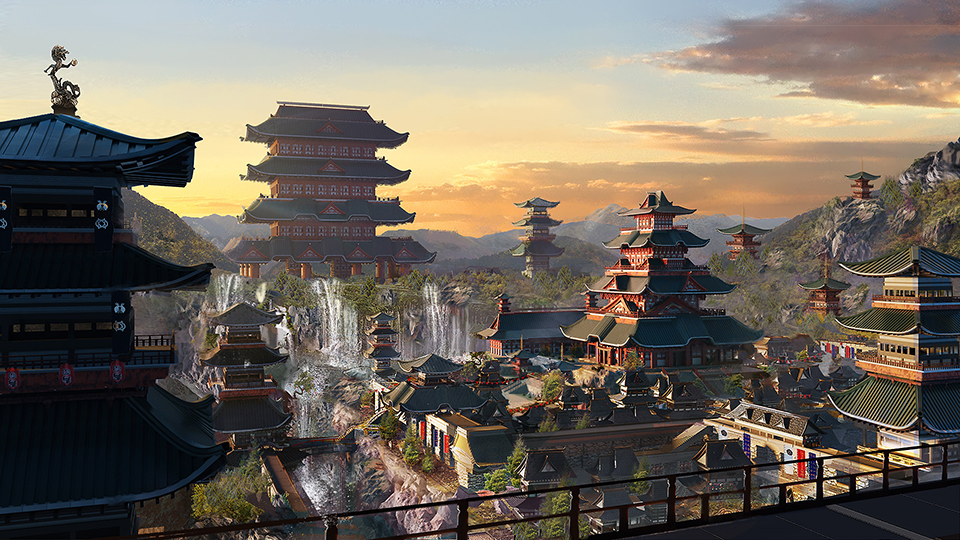
\includegraphics[width=\linewidth]{bilder/Konzept}}
  \caption{Konzept für Farbgebung und Aufbau der Gebäude \parencite{JapanConcept}.}
	\label{JapanKonzept}
\end{figure}
\newpage
Nach der konzeptionellen Planung wurde geprüft, welche Möglichkeiten die genutzten Programme bieten, um das Projekt umzusetzen. Zudem wurden erste Einstellungen vorgenommen, um einen fehlerfreien Ablauf nachfolgender Prozesse zu gewährleisten. Die Maßeinheiten von Blender und Unreal Engine wurden aufeinander abgestimmt und die \textit{Snapping}-Funktion in Unreal Engine getestet.\footnote{\,Für dieses Projekt wurde mit Blender 2.79b und Unreal Engine 4.21.2 gearbeitet}
\par
In Unreal Engine wurde bisher mit Zentimetern gearbeitet, dies wird so beibehalten. Für das Arbeiten mit einem modularen System wird das Raster von klassisch (mit Schritten von 1 m, 2 m, 5 m usw.) auf die Basis von zwei und dessen Potenzen eingestellt. Abstände, die so entstehen, lassen sich, wie in Abschnitt \ref{Rasterkapitel} erwähnt, besser halbieren ohne das ungerade Zahlen entstehen, die das genaue Platzieren von Objekten deutlich erschweren würden. Durch eine einfache Einstellung im Viewport\footnote{\,Der Viewport ist eine grafische Oberfläche, in dem das aktuelle Level betrachtet und bearbeitet werden kann} kann die Raster Größe (2 cm, 4 cm, 8 cm, ... 128 cm, 256 cm, usw.) angepasst werden.
\par
Auch in Blender kann die Maßeinheit auf Zentimeter eingestellt und das selbe Raster wie in Unreal Engine gewählt werden. Das Raster wird hier allerdings nur wenig benutzt: Beim Modellieren ist es eher hinderlich, wenn Bewegungen nur in definierten Schritten durchgeführt werden können, da viele Details der Modelle dem Raster nicht folgen werden.
\par
Die Planung der Elemente basiert auf den Eigenschaften bestehender Assets. Durch dieses Vorgehen soll sichergestellt werden, dass sich die neuen Modelle in den bestehenden Stil einfügen.
\par
Die bisherigen Gebäude wurden für ein anderes Setting entwickelt, die genutzten Maße gelten dennoch als Orientierung für die neuen Assets.
\newpage
\begin{description}
\item[Größen bestehender Elemente]\hfill
\begin{itemize}[leftmargin=0cm]
\item Türen sind 2,8 m hoch und 1,8 m breit,
\item Fenster sind zwischen 1,5 m und 2,4 m hoch und breit,
\item eine Etage der alten Gebäude ist ca. 4,3 m hoch,
\item Treppenstufen an Gebäuden haben eine Höhe  von ca. 24 cm und eine Tiefe von ca. 27 cm,
\item Treppenstufen in der Welt haben eine Höhe  von ca. 42 cm und eine Tiefe von ca. 56 cm und
\item die Spielfiguren sind 195 cm hoch und ca. 70 cm breit.
\end{itemize}
\end{description}
Als Fußabdruck (siehe Abschnitt \ref{Rasterkapitel}) für die neuen Elemente wird eine Größe von 5,12 m x 5,12 m x 5,12 m genutzt. Kein erstelltes Element soll den so definierten Würfel überschreiten.
\par
Auf Grundlage der bestehenden Gebäude wurde sich für eine Etagenhöhe von 5,12 m entschieden. Grund hierfür war die ursprüngliche Etagenhöhe von 4,3 m, zu der für die neuen Gebäude noch die Höhe des Vordaches addiert wird. Nach längerer Planung habe ich mich für Elemente entschieden, die so aufgebaut sein sollen, wie in Abbildung \ref{KitelementeSkizze} eingezeichnet. In der Modelierungsphase wurde erkannt, dass dieser Ansatz eher ungeeignet ist um das volle Potenzial von Modularität auszunutzen. Im nächsten Abschnitt wird auf den alternativen Lösungsansatz eingegangen.
\par
Damit das Kit mehr Abwechslung erzeugen kann, wurden zudem Elemente in halber Höhe (2,56 m) und halber Breite (2,56 m) geplant. Ein schon in der Planungsphase erkennbares Problem, war das Zusammenlaufen der Etagen. Der Prozess zur Lösung dieses Problems wurde in die Modellierungsphase verschoben. Es erschien leichter, eine Lösung im dreidimensionalen Raum zu finden, statt mit Skizzen zu arbeiten.
\begin{figure}[!h]
\centering
  \makebox[\textwidth]{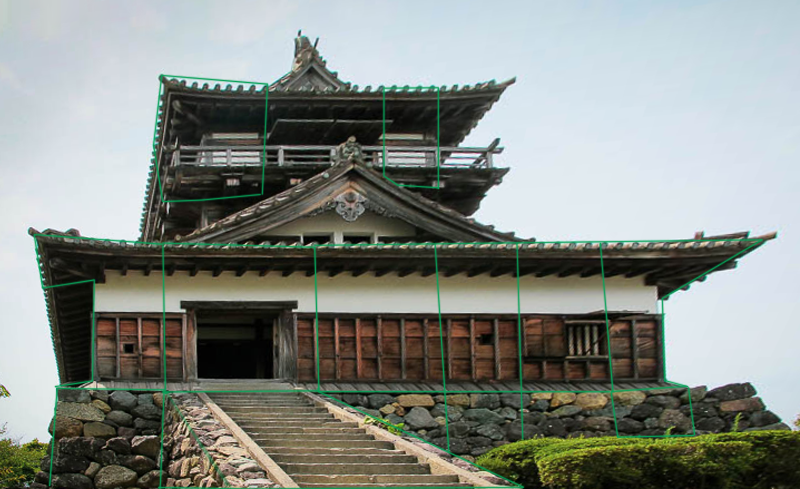
\includegraphics[width=0.8\linewidth]{bilder/KitelementeSkizze}}
  \caption{Skizze der zunächst definierten Module. In Anlehnung an \parencite{KitelementeSkizze}.}
	\label{KitelementeSkizze}
\end{figure}
\newpage
Für das Projekt wurde eine mittlere Stufe von Modularität gewählt. Weitere Varianz wird durch verschiedene Versionen der gleichen Elemente erzeugt. Zusätzlich werden kleinere Module erstellt, um Muster aufzubrechen und den Gebäuden mehr Details zu verleihen. Bisher wurden neun verschiedene Gebäude für alle Level genutzt, aufgrund der Perspektive und der Art des Gameplays ist dies bisher nur gering negativ aufgefallen. Folglich sollte es unproblematisch sein, wenn die neuen Gebäude, aus der genutzten Spielperspektive, aus größeren Elementen bestehen, auch wenn es weniger Abwechslung bedeutet.
\par
Das Kit wurde für eine bessere Übersicht und leichtere Handhabung in sieben Subkits aufgeteilt. Die Sets entsprechen jeweils einer Ebene des Gebäudes.
\begin{table}[H]
\fontsize{9}{11}\selectfont
\centering
\begin{tabular}{| l | l |}
\hline\par
\textbf{Subkit}&\multicolumn{1}{c |}{\textbf{Bedeutung}}\\ \hline
Fundament&Elemente für das optionale Steinfundament \\ \hline
Wall&Wandelemente\\ \hline
Balcony&Balkonelemente\\ \hline
Roof&Elemente für das optionale Dach\\ \hline
TopRoof&Dachelemente\\ \hline
Joist&Dachbalkenelemente, die auf das Dach gesetzt werden können\\ \hline
Beam&Holzbalkenelemente, die an Wandübergängen platziert werden können\\ \hline
\end{tabular}
\caption{Übersicht aller Subkits und deren Bedeutung}
\end{table}
\vspace{-10.5pt}
Die Benennung der Elemente, ist wie in Abschnitt \ref{Kit Spezifische Planung} erwähnt, ein wichtiger Faktor für effizientes Arbeiten mit modularen Kits. Für die Bezeichnung wurden verschiedene Begriffskategorien definiert, mit deren Hilfe die Elemente genau zugeordnet werden können. Der Name eines Moduls setzt sich aus den folgenden Kategorien zusammen:
\begin{table}[H]
\fontsize{9}{11}\selectfont
\centering
\begin{tabular}{ l  l  l  l  l }
Subkit & Höhe & Form & Breite & Variante\\ \hline
Ro(of) & Ha(lf) & In(ner Corner) & Si(ngle) & 04
\end{tabular}
 \caption{Bezeichnungsschemata der genutzten Module mit einem Beispiel}
\end{table}
\vspace{-10.5pt}
Zuerst wurde versucht die Bezeichnungen der Elemente nur aus den Anfangsbuchstaben der Wörter zu bilden, die ein Modul ausmachen (z. B. \enquote{FSBS01}). Es stellte sich heraus, dass eine so starke Vereinfachung schwer zu lesen beziehungsweise zu erlernen ist. Aus diesem Grund wurden für die Benennung der Elemente die ersten beiden Buchstaben genutzt, um die Namen der Elemente zu generieren. Aus \enquote{FSBS01} wurde \enquote{FuSiBaSi01}, welches einfacher in \enquote{Fundament Single Basic Single 01} übersetzt werden kann.
\par
Die Bezeichnung der Höhe wurde so weit vorne im Namen platziert, damit bei einer Suche im Editor zusammengehörige Elemente leicht gefunden werden können. Die verschieden hohen Elemente können auf einer Ebene nicht miteinander verbunden werden. Durch dieses Schema können die nicht kompatiblen Elemente leicht voneinander getrennt werden.
\par
Der Abschnitt zur Planung ist hier beendet, die Planung insgesamt jedoch noch nicht und wird während der Modellierung fortgeführt. Die geplanten Konzepte müssen mit einfachen Modellen getestet und eventuell angepasst werden. Nur so können im späteren Verlauf Fehler vermieden werden.
\enlargethispage{10.5pt}
\subsection{Modellierung}
Zu Beginn der Modelierungsphase wurden Prototypen der konzipierten Modelle erstellt und auf ihre Funktion hin überprüft.
\par
Das zuvor entwickelte System funktionierte. Durch das Einhalten der definierten Größen und das Platzieren der Pivot Points an den unteren Eckpunkten der Module ließen sich die Objekte leicht miteinander verbinden ohne das Lücken entstanden.
\par
Um zu überprüfen, ob das Kit auch in der Unreal Engine funktioniert, wurden die Module testweise importiert und zu einem Gebäude verbunden (Abbildung \ref{ErsterTestInUnreal}). Auch in der Engine traten keine Probleme mit dem Kit auf. Das Raster in Unreal Engine wurde auf 1.28 m eingestellt, was das Zusammensetzen des Gebäudes enorm beschleunigt.
\begin{figure}[H]
\centering
  \subfloat[][Alle Prototypen-Module in Blender.]{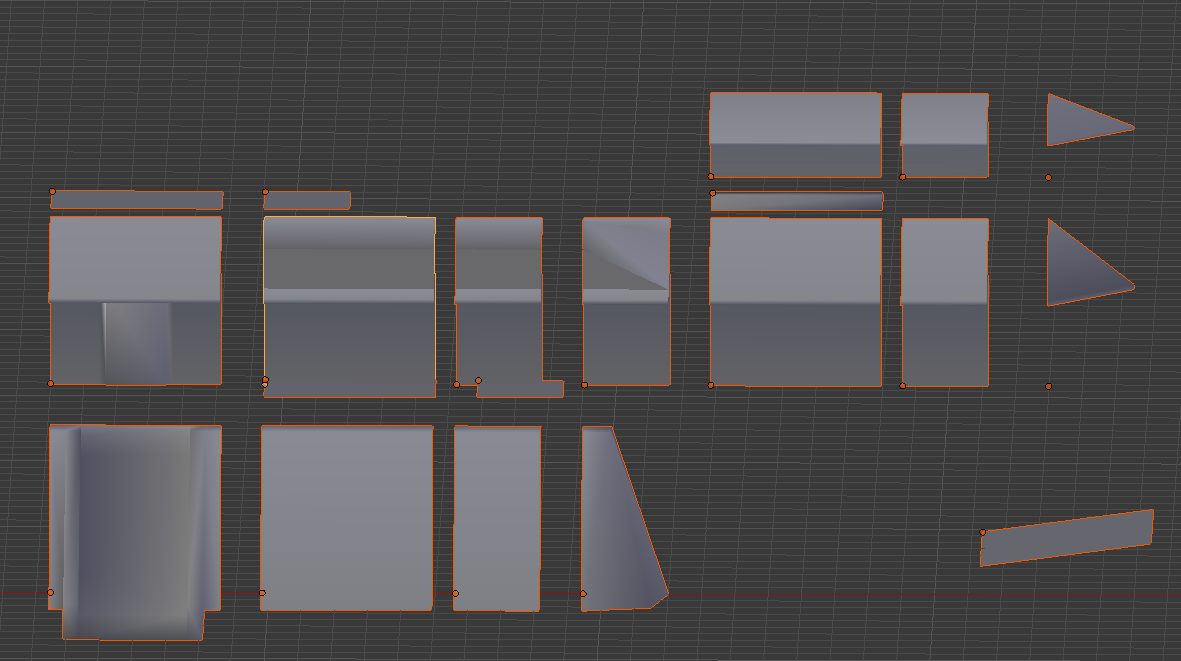
\includegraphics[height=4.2cm]{bilder/ErsterModulTest}\label{ErsterModulTest}}%
  \qquad
  \subfloat[][Aus Modulen erstelltes Gebäude in Unreal Engine.]{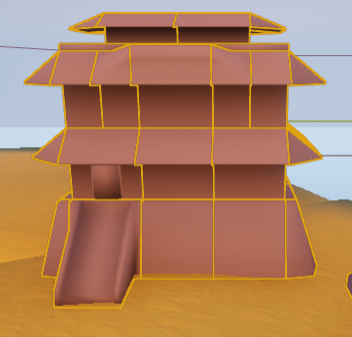
\includegraphics[height=4.2cm]{bilder/ErsterTestInUnreal}\label{ErsterTestInUnreal}}%
  \caption{Erste Prototypen der geplanten Module.}%
\label{ErsterModulTest}
\end{figure}
\vspace{-10.5pt}
\begin{wrapfigure}{l}{0.5\textwidth}
  \centering 
  \vspace{-11.5pt}
    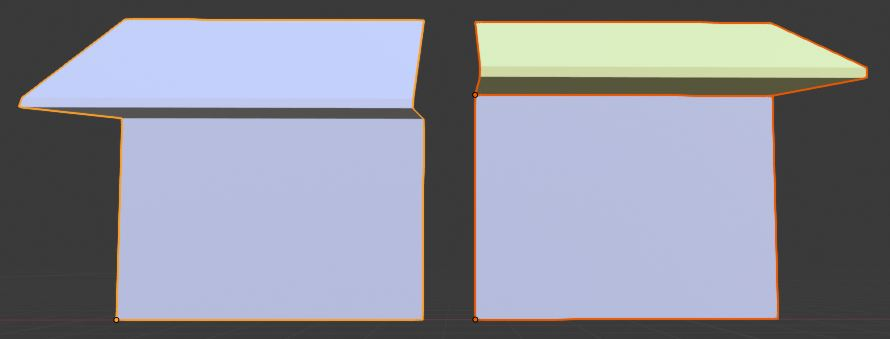
\includegraphics[width=0.5\textwidth]{bilder/Wallrework}
      \caption{Ursprüngliches Wandelement (links) und überarbeitete Version mit abgelöstem Dach (rechts).}\label{Wallrework}
          \vspace{-10pt}
\end{wrapfigure}
Im Anschluss wurde begonnen, die Module weiter auszubauen. Dabei wurde klar, dass die geplante Struktur der Module die Modularität des Kits vermindern und den Arbeitsaufwand vergrößern würde. Es war geplant, dass jedes Wandmodul mit einem Dach oder einem Dach und einem Balkon erstellt werden sollte. Ein besserer Ansatz ist es, die Dächer und Balkone von den Wänden zu trennen, was zur Folge hat, dass die Wände nicht mehr eine Höhe von 5,12 Metern haben. Um das Raster nicht zu verlassen, wurde die normale Größe von Wänden auf 3,84 Metern gesetzt. Zusammen mit Dachelementen, die 1,28 Meter hoch werden, kann die Etagenhöhe von 5,12 Metern wieder eingehalten werden. Die zuvor geplanten halbhohen Wandelemente werden mit einer Höhe von 2,56 Metern erstellt. 
\newpage
\begin{wrapfigure}{l}{0.35\textwidth}
\centering 
  \vspace{-0.5pt}
    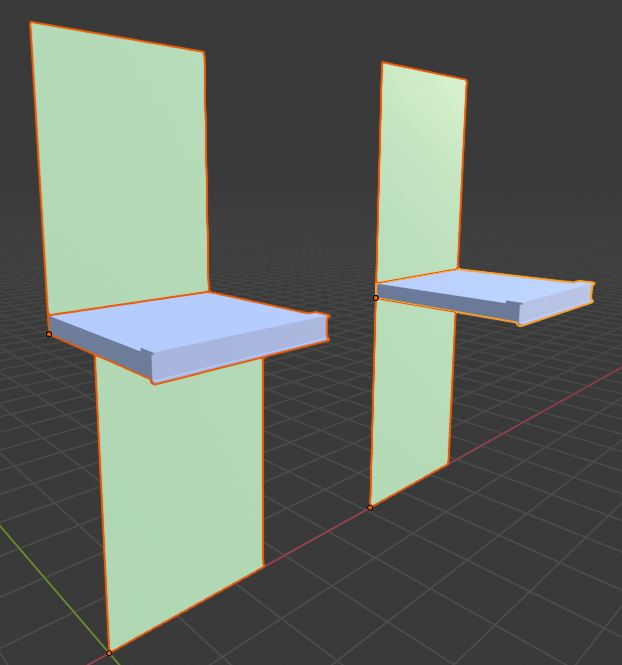
\includegraphics[width=0.35\textwidth]{bilder/balconposition}
      \caption{Mögliche Kombinationen von Balkon- und Wandelementen.}\label{balconposition}
      \vspace{-14pt}
\end{wrapfigure}
Durch diese Änderung konnte die Anzahl der benötigten Module verringert und die Modularität des Kits erhöht werden. Bei Bedarf können Wandelemente auch ohne Dachelemente aufeinander gesetzt werden, um größere Wände zu erzeugen. Auch Balkonmodule können durch diese Entwicklung vielseitiger genutzt werden. Sie können entweder an die Wand gesetzt werden oder auch 1,28 Meter nach innen in das Gebäude verschoben werden, um die nachfolgende Etage zu verkleinern, ohne dass hierfür verschiedene Module benötigt werden.
\par
\begin{wrapfigure}{l}{0.35\textwidth}
\centering 
  \vspace{-11.5pt}
    \includegraphics[width=0.35\textwidth]{bilder/holzecke}
      \caption{In Wandelemente eingesetzte Holzbalken mit Sonderelement.}\label{holzecke}
      \vspace{-14pt}
\end{wrapfigure}
Nach der Überarbeitung des Systems wurden die neuen Wandelemente mit einem halben vertikalen Holzbalken am linken und rechten Rand erweitert. Werden zwei Elemente miteinander verbunden, bildet sich am Übergang ein vollständiger Holzbalken. Die Holzbalken wurden eingesetzt, um das Kit dem Setting anzupassen. Wurde mit Wandmodulen eine Ecke gebildet, entstand eine Lücke zwischen den Holzbalken, die mit einem Sonderelement gefüllt werden musste.
\par
Bei einem weiteren Test in Unreal Engine wurden Probleme mit Schatten gefunden. An Stellen, bei denen Module aufeinander treffen und keinen glatten Übergang bilden, kommt es zu sehr starken Helligkeitsunterschieden, die falsch aussehen. Dies passierte bei dem Element zum Füllen der Lücke zwischen Holzbalken und bei der bis dahin genutzten Form von Eckelementen der Dachmodule. Dieses Problem kann auch bei glatten Übergängen auftreten, ist dort aber weniger auffällig.
\par
Die Form der Dachmodule wurde daraufhin so abgeändert, dass die Übergänge zu geraden Modulen eine glatte Fläche bilden.
\par
\begin{wrapfigure}{l}{0.35\textwidth}
  \centering 
   \vspace{-11.5pt}
    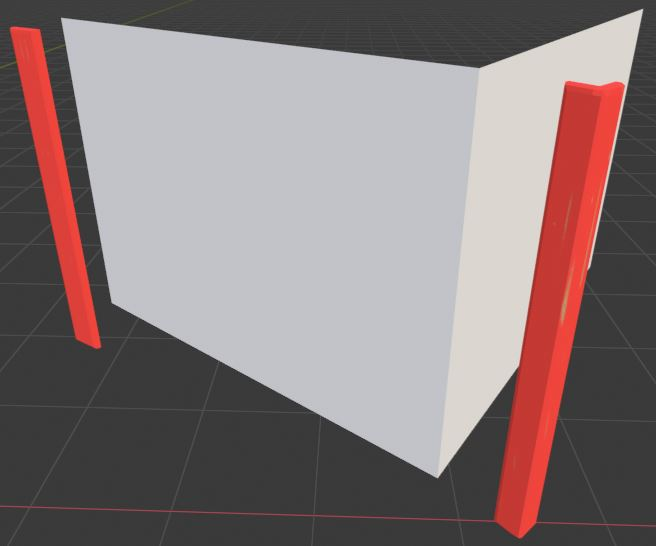
\includegraphics[width=0.35\textwidth]{bilder/holzecke2}
      \caption{Überarbeitete Wandelemente und Holzbalken aus neuem Subkit.}\label{holzecke2}
          \vspace{-14pt}
\end{wrapfigure}
Die zuvor in die Wände eingesetzten Holzbalken wurden wieder von den Wänden gelöst und wurden in ein eigenes Subkit verschoben. In diesem Subkit gibt es Holzbalken für die verschiedenen hohen Module und auch für Außen- und Innenecken. Durch diese Änderungen wurden die Probleme mit den Schatten gelöst. Zusätzlich können so verschiedene Versionen von Holzbalken genutzt werden, wodurch eine sichtbare Wiederholung vermindert wird. Auch ist es möglich Wände ohne Holzbalken zu bilden, was weitere Möglichkeiten eröffnet.
\newpage
Nach diesen Anpassungen wurden weitere Tests durchgeführt. Bei diesen wurde festgestellt, dass offenbar bei einer bestimmten Kombination von Dach- und Balkonelementen im Dach Lücken entstehen können, die nicht mit bestehenden Modulen gefüllt werden können. Die Lücken hatten eine Breite von 1,28 Metern, dies entspricht einem Viertel der normalen Breite aller Elemente.
\par
\begin{wrapfigure}{l}{0.4\textwidth}
  \centering 
   \vspace{-12.5pt}
    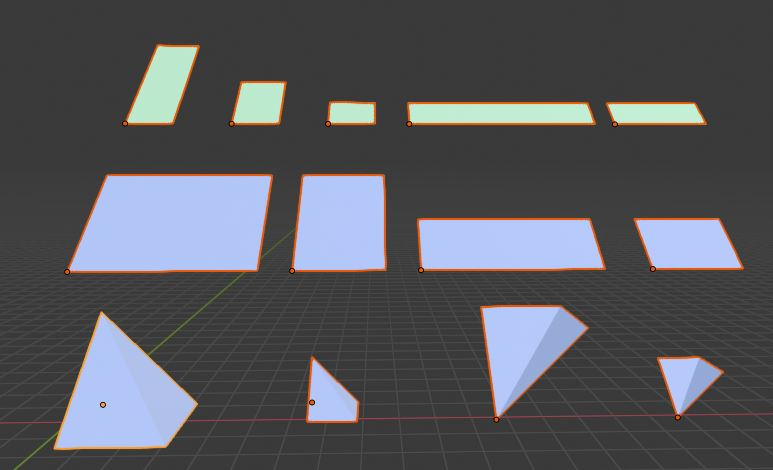
\includegraphics[width=0.4\textwidth]{bilder/DacheElemente}
      \caption{Ursprüngliches Elemente für den Abschluss des Daches (blau) und neue Elemente für das schließen spezifischer Lücken (grün).}\label{DacheElemente}
          \vspace{-14pt}
\end{wrapfigure}
Nach mehreren erfolglosen Versuchen diese Lücken ,ohne viele neue Elemente zu vermeiden, wurde dem Subkit, für die Schließung des Gebäudes, weitere Elemente hinzugefügt. Auf Basis der bestehenden Elemente wurden neue Elemente in verschiedenen Kombinationen aus einem Viertel der Höhe und einem Viertel der Breite erstellt.
\par
Mit diesen neuen Modulen war das Kit vollständig (Abbildung \ref{finalmodul}) und alle Modelle konnten weiter ausgearbeitet werden.
\begin{figure}[H]
\centering
  \makebox[\textwidth]{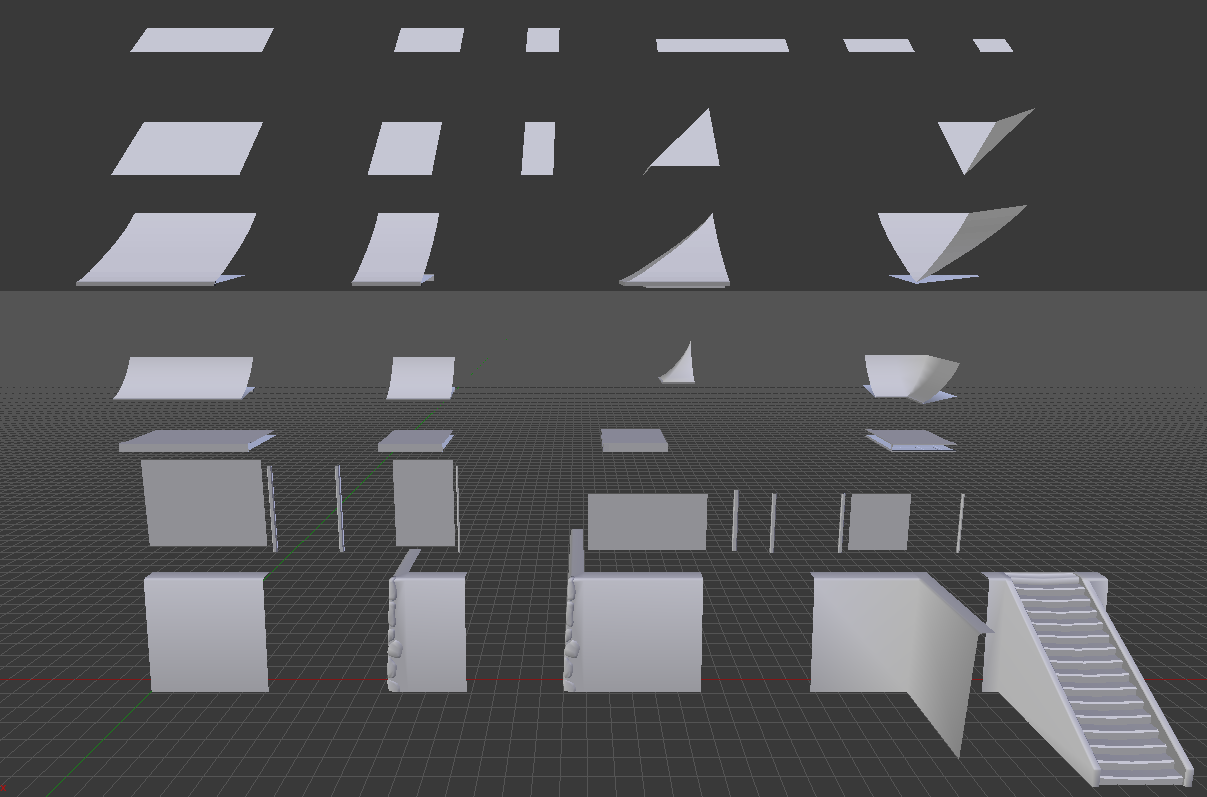
\includegraphics[width=1\linewidth]{bilder/Prototypen2}}
  \caption{Prototypen des weiterentwickelten Systems.}
	\label{finalmodul}
\end{figure}
\vspace{-10.5pt}
Die finalen Module wurden von unten nach oben entwickelt. Zuerst wurde das Fundament fertiggestellt, dann die Wände, die Vordächer, die Balkone und zum Schluss die Dachelemente, die das Gebäude abschließen. Auf diese Weise konnte immer überprüft werden, ob die neuen Elemente ohne Probleme auf die unterliegende Schicht passen.
\par
Aufgrund der speziellen Architektur der Gebäude konnte keine vollständige Modularität erreicht werden. Module sind horizontal immer nur mit Modulen des gleichen Subkits kombinierbar. Vertikal können alle Subkits miteinander verbunden werden. Ausschließlich das Fundament-Subkit kann nur als unterste Ebene fungieren, da es auf Grund seiner speziellen Form nicht auf andere Elemente gesetzt werden kann.
\begin{figure}[H]
\centering
  \makebox[\textwidth]{\includegraphics[width=1\linewidth]{bilder/AllModules}}
  \caption{Alle Module mit angewandten Texturen.}
	\label{alleModule}
\end{figure}
\vspace{-10.5pt}
Für das Projekt wurden insgesamt 76 verschiedene Elemente erzeugt. Von den Wand-, Balkon- und Holzbalkenelementen wurden zusätzliche Varianten erzeugt, um eine abwechslungsreichere Gestaltung zu ermöglichen. Zusammen mit diesen entstanden insgesamt 126 Module. Abbildung \ref{alleModule}, zeigt alle erstellten Module in ihrem finalen Zustand.
\newpage
\subsection{Texturierung}
Wie zuvor erwähnt, steht in dieser Arbeit die Erstellung der Modelle im Vordergrund; infolgedessen wird in diesem Abschnitt nur skizziert, wie für die Texturierung vorgegangen wurde.
\par
Nach der Planungsphase wurde für alle benötigten Texturen eine Vorabversion erstellt. So konnten für die Modelle schon passende UV-Maps erstellt werden. Hier war zu beachten, dass die Ränder der Modelle mit den Rändern der Textur verbunden wurden. Nur so kann ein nahtloser Übergang zwischen Modulen gewährleistet werden. Durch das Texturieren der Modelle konnte schon früh ein Eindruck vermittelt werden, wie die Module später aussehen werden. Die finale Version der Texturen wurde nach Abschluss der Modellierphase erstellt.
\par
Um zu erfahren, welche verschiedenen Texturen benötigt werden, wurden Bilder der nachzubildenden Gebäude auf genutzte Baumaterialien hin analysiert. Zusammen mit dem vorliegenden Konzept (Abblidung \ref{JapanKonzept}) konnte so eine Liste mit benötigten Texturen ausgearbeitet werden.
\begin{figure}[H]
\centering
  \subfloat[][Steintextur für Fundamentelemente.]{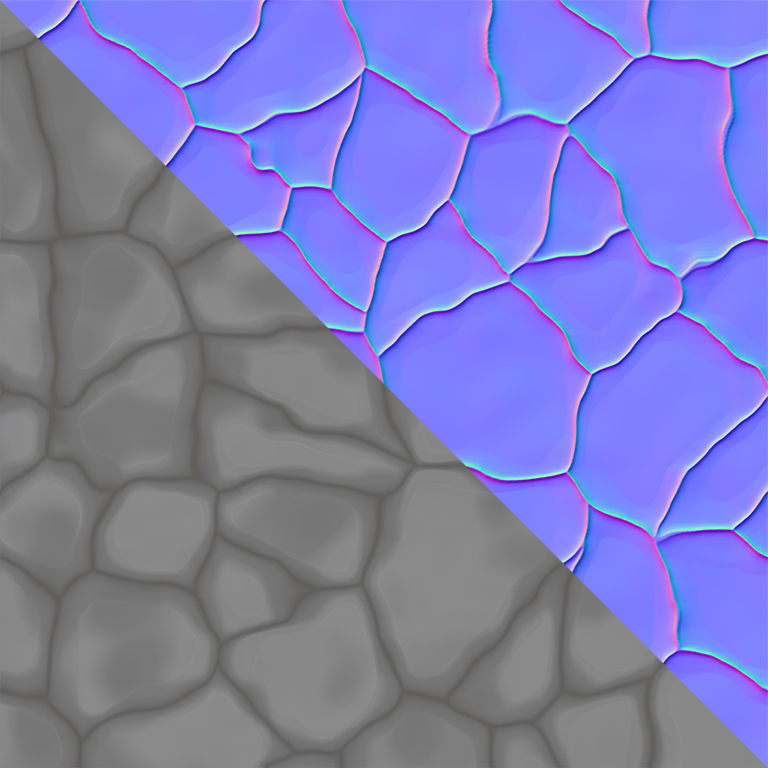
\includegraphics[width=0.29\linewidth]{bilder/StoneWall}\label{StoneWall}}%
  \qquad
  \subfloat[][Steintextur für Treppenstufen.]{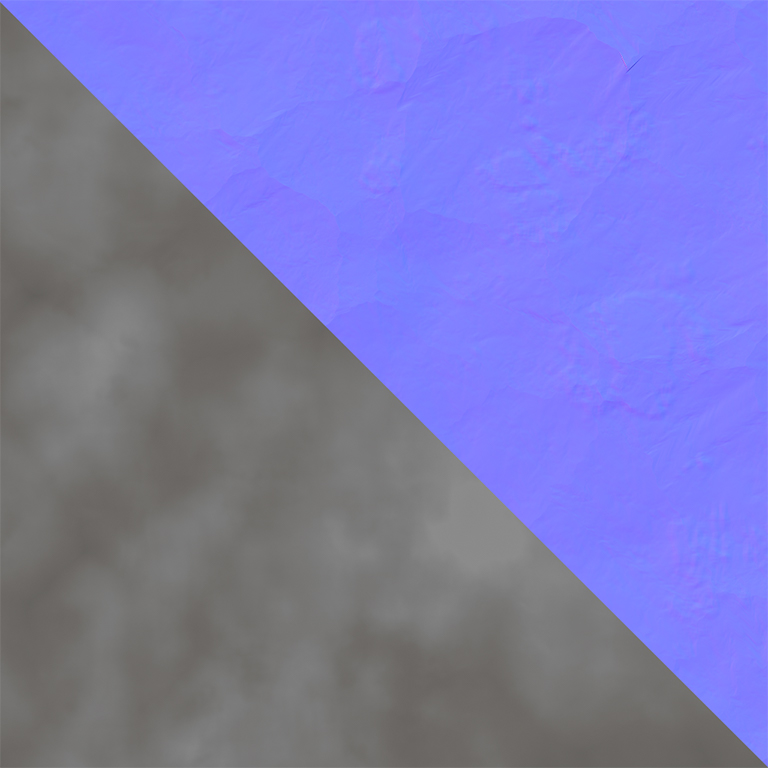
\includegraphics[width=0.29\linewidth]{bilder/StoneStairs}\label{StoneStairs}}%
   \qquad
  \subfloat[][Dachziegeltextur für Dachelemente.]{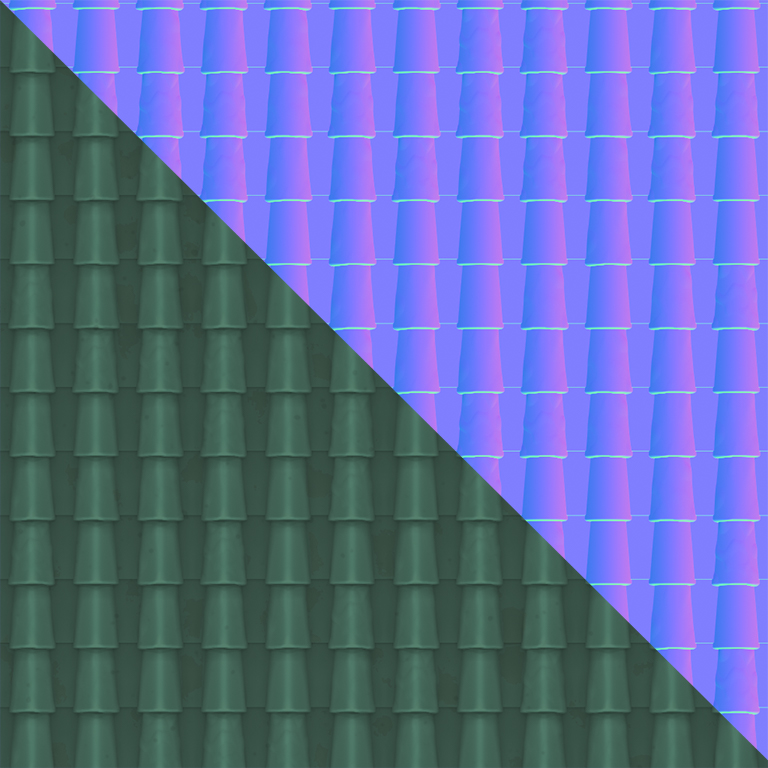
\includegraphics[width=0.29\linewidth]{bilder/RoofTiles}\label{RoofTiles}}%
   \qquad
  \subfloat[][Holztexturen für Holzelemente.]{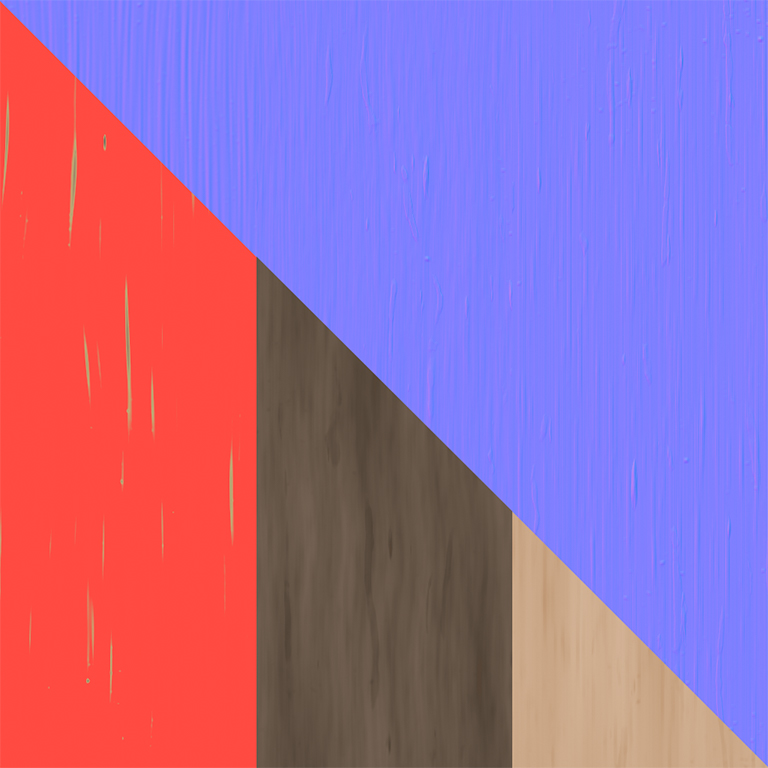
\includegraphics[width=0.29\linewidth]{bilder/Wood}\label{Wood}}%
   \qquad
  \subfloat[][Steintextur für Wandelemente.]{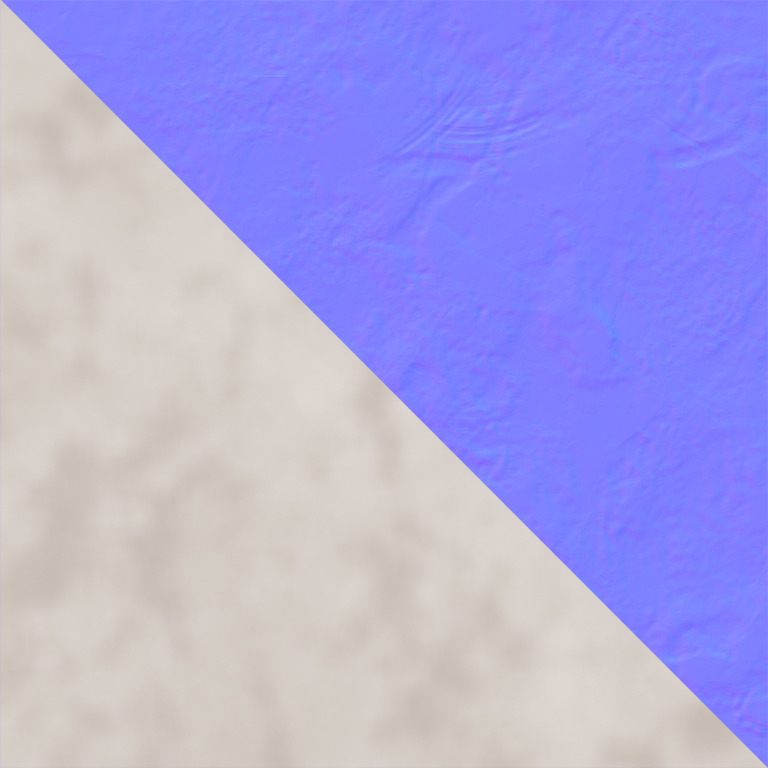
\includegraphics[width=0.29\linewidth]{bilder/WhiteWall}\label{WhiteWall}}%
   \qquad
  \subfloat[][Papiertextur für Fenster.]{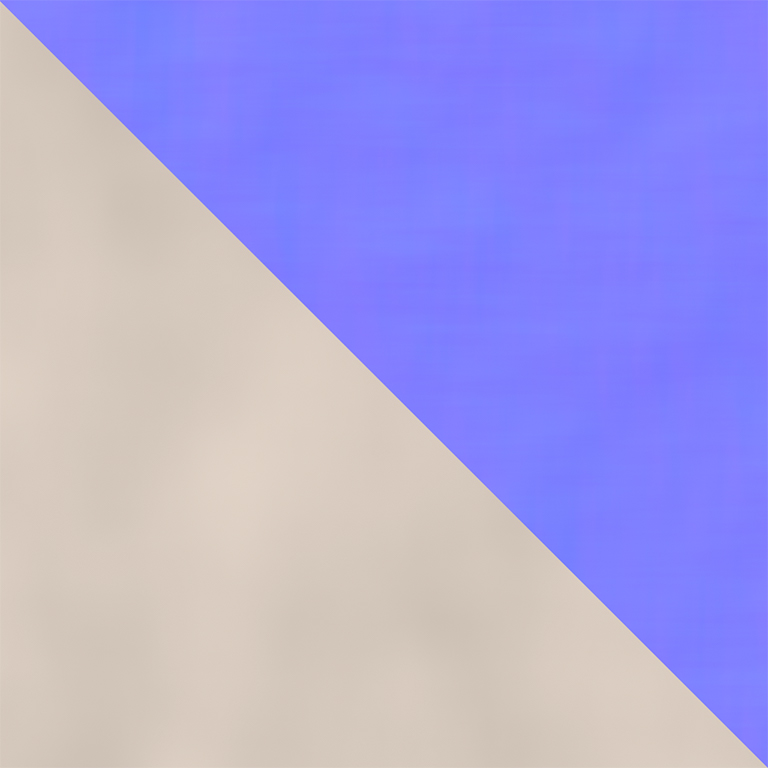
\includegraphics[width=0.295\linewidth]{bilder/Paper}\label{Paper}}%
  \caption{Ausschnitte aller benötigten Diffuse- und Normalmaps.}%
\label{Textures}
\end{figure}
\vspace{-10.5pt}
Im Anschluss wurden alle Texturen mit \textit{Substance Designer} erstellt. Werden Texturen mit den Standardeinstellungen von \textit{Substance Designer} erstellt, sind diese immer so ausgelegt, dass sie in alle Richtungen kachelbar sind. Dies ist für modulare Assets sehr wichtig, um an Übergängen zwischen Modulen sichtbare Kanten zu vermeiden.
\begin{figure}[H]
\centering
  \subfloat[][Specularmap.]{
\includegraphics[width=0.34\linewidth]{bilder/specular}\label{specular}}%
  \qquad
  \subfloat[][Rougnessmap.]{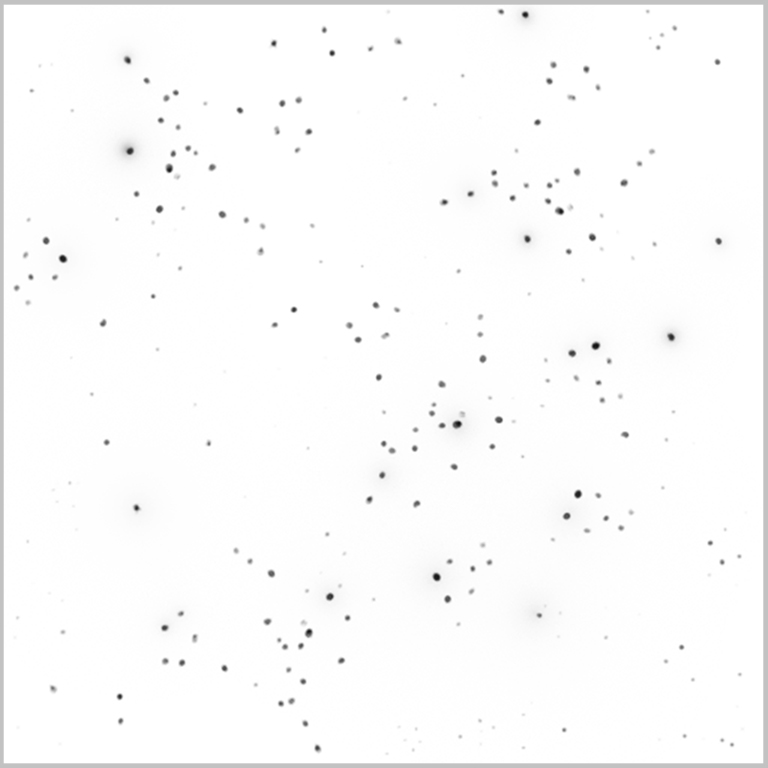
\includegraphics[width=0.34\linewidth]{bilder/roughness}\label{roughness}}%
  \caption{Die für die meisten Modelle genutzten Rougness- und Specularmaps.}%
\label{altemaps}
\end{figure}
\vspace{-10.5pt}
In \textit{Renegade Line} werden für die Materialien Albedo-, Normal-, Roughness- und Specularmaps genutzt. Die Roughness- und Specularmap werden von den bestehenden Modellen übernommen. Diese sind größtenteils einfarbig und sorgen für ein eher stumpfes Erscheinungsbild der Modelle. Dies ist für den angestrebten Cartoon Look sehr wichtig. Die Albedo- und Normalmap wurde für jede Textur von Grund auf neu erzeugt. Für die Griffe an den Türen wurde ein schon existierendes Metall Material genutzt.
\begin{figure}[H]
\centering
  \makebox[\textwidth]{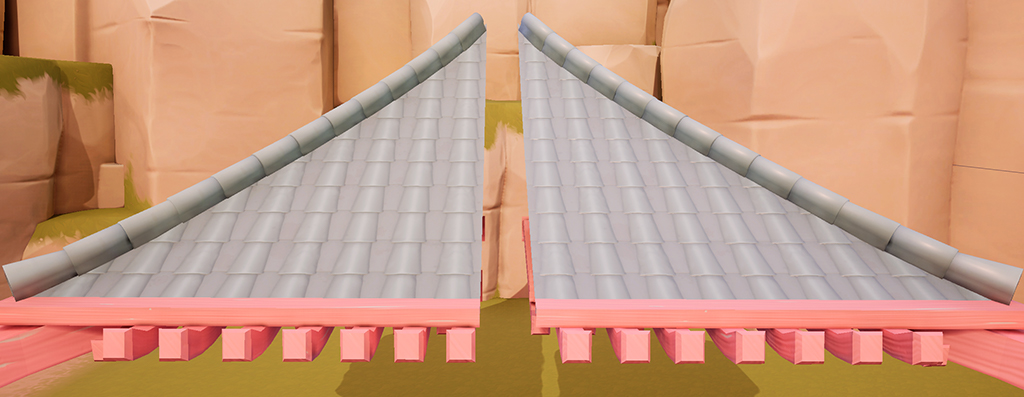
\includegraphics[width=\linewidth]{bilder/specroughvs}}
  \caption{Einfluss der Specular- und Roughnessmap (links) im Vergleich mit den Standartwerten aus Unreal Engine (rechts).}
	\label{specroughvs}
\end{figure}
\vspace{-10.5pt}
Von den Holztexturen für Holzbalken und Leisten an Türen, Fenstern und Dächern wurden drei Versionen erstellt: Eine, zum Konzept passende Rote sowie eine mit hellem und eine mit dunklem Holz (Abbildung \ref{Wood}). So kann ein Gebäude durch Tausch einer Textur einen ganz neuen Look erhalten.
\par
Versuche einen Texturatlas zu nutzen wurden nach Tests in Unreal Engine nicht weiter verfolgt. Durch Mip Mapping, ein Vorgang bei dem Texturen komprimiert werden, um eine bessere Spielperformance zu gewährleisten, wurden nebeneinander liegende Texturen vermischt. Diese Vermischung führte zu sichtbaren Kanten auf den Modellen. Zusätzlich wäre es komplizierter gewesen die verschiedenen Holzarten zu nutzen, wenn diese nicht in verschiedene Materialien aufgeteilt worden wären.!!!
\subsection{Implementierung}\label{implementierung2}
Nachdem alle Tests bezüglich der Funktion und des Aussehens des Kits abgeschlossen waren, wurden alle Testdateien aus dem Unreal Engine-Projekt entfernt.
\par
Im Anschluss wurden für Texturen, Materialien, Modelle und fertige Gebäude Ordner angelegt. Der Ordner für die Modelle wurde mit Unterordnern für die Subkits gefüllt. Die fertigen Modelle sollten in Blueprints\footnote{\,In Unreal Engine sind Blueprints eine Art leerer Container der Code ausführen und Objekte enthalten kann} abgespeichert und in dem dafür vorgesehenen Ordner gesichert werden.
\par
Zuerst wurden alle Texturen importiert und auf deren Grundlage neue Materialien erstellt. Dann wurden die Modelle importiert und jedem Modell wurde ein Standardset an Materialien zugeordnet. Alle Modelle mit Holzelementen wurden mit dem roten Holz ausgestattet, dessen Verwendung als Preset vorgesehen ist.
\par
Nach der Implementierung wurden für  Tests erste Gebäude in Unreal Engine erstellt. Die schon zuvor festgestellten Belichtungsprobleme an glatten Übergängen konnten durch Anpassungen der Lichtberechnung in den Welteinstellungen und dem Vergrößern der Lightmap gelöst werden. Die Lightmap ist ein Bild in der die Schattenwerte gespeichert werden, die durch die Berechnung des Lichtes ermittelt wurden. Die Modelle nutzen nun eine Lightmap-Größe von 128 x 128 Pixeln. Die vorkonfigurierten 64 x 64 Pixel waren zu klein und führten an manchen Stellen zu Überlappungen zwischen den Faces.
\begin{figure}[H]
\centering
  \makebox[\textwidth]{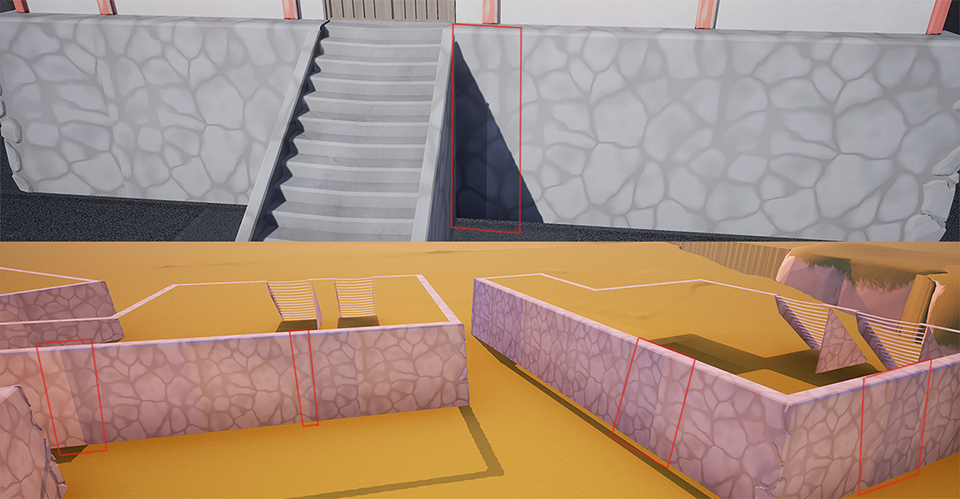
\includegraphics[width=\linewidth]{bilder/LichtProblem}}
  \caption{Harte Kanten an Modulübergängen von Modulen.}
	\label{LichtProblem}
\end{figure}
\vspace{-10.5pt}
Das Ändern der Lichtberechnungseinstellungen verlangsamte die Lichtberechnung. Da dieser Prozess vor dem Spielen ausgeführt wird, hat dies keinen negativen Einfluss auf die Spielperformance, erhöht aber die Dauer von Tests in der Entwicklung. Nachdem die Probleme der Beleuchtung gelöst waren, wurden weitere Gebäude erstellt.
\newpage
Während dessen wurden keine Probleme festgestellt. Alle Module konnten wie geplant ohne Fehler verbunden werden. So wurden zehn verschiedene Gebäude erstellt, um mögliche Formen und Größen der Gebäude zu testen. Um zu überprüfen, ob sie beziehungsweise das modulare Kit in die alte Spielwelt passen, wurden die Gebäude in ein bestehendes Level eingefügt.
\begin{figure}[H]
\centering
  \makebox[\textwidth]{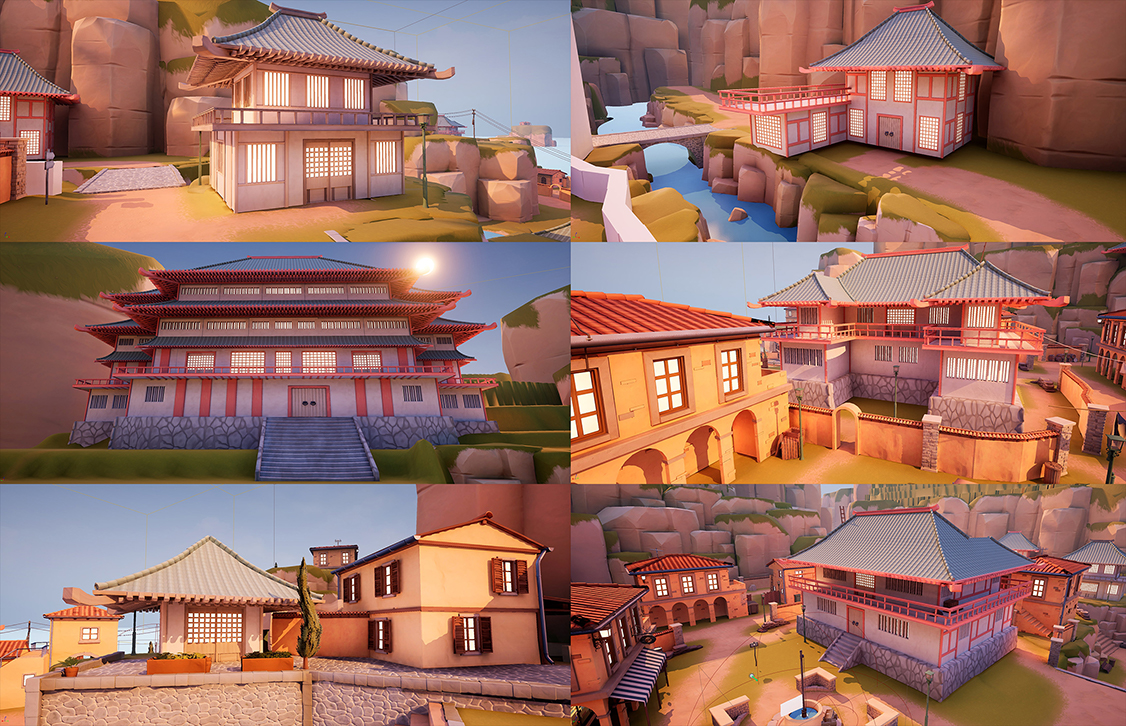
\includegraphics[width=\linewidth]{bilder/StilTest}}
  \caption{Aus dem Kit erstellte Gebäude in einem alten Level.}
	\label{stilTest}
\end{figure}
\vspace{-10.5pt}
Die neuen Gebäude fügen sich sehr gut in den bestehenden Spielstil ein, auch wenn die übrigen Assets ein anderes Setting repräsentieren. Das an dem Spiel beteiligte Team war sich über die Diskussion der Ästetik hinaus einig, dass die neuen Gebäude zu dem bestehenden Stil passen.
\par
Für die Bewertung des Kits wurde ein Performance-Test durchgeführt, der ernüchternde Ergebnisse lieferte.
\par
Die Tests wurden auf einem sehr leistungsstarken Desktop-PC\footnote{\,Der PC ist aus folgenden Komponenten zusammengesetzt: INTEL CORE i7-4790K 4.0GHz, GeForce GTX 970 4GB Grafikkarte, 16GB Arbeitsspeicher und 1TB HDD Festplatte.} durchgeführt. 
\par
Es wurden zwei verschiedene Gebäude in zwei Versionen für die Tests genutzt: Jeweils eine, aus Modulen in Unreal Engine zusammengesetzte Version und eine, die in Blender erstellt und als ein einzelnes Objekt in Unreal Engine importiert wurde. Ein Gebäude ist einfach aufgebaut und soll vielfach in einem Level auftauchen. Während des Spielens sieht der Spieler ungefähr zehn der einfach aufgebauten Gebäude auf einmal, diese Zahl kann je nach Level und Position des Spielers variieren. Das andere Gebäude ist größer und komplexer aufgebaut, es repräsentiert eine Art Palast der pro Level nur einmal vorkommen soll.
\newpage
Die Komplexität der Modelle lässt sich wie folgt darstellen:
\begin{table}[H]
\fontsize{9}{10}\selectfont
\begin{tabular}{ p{0.094\textwidth} |  p{0.407\textwidth} |  p{0.407\textwidth} }
\vspace{74pt}Kleines \newline Gebäude &
\vspace{0.2pt}
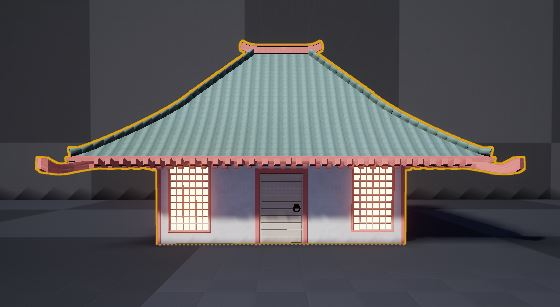
\includegraphics[width=\linewidth]{bilder/smallhousepiece}\newline
26.000 Triangles, 7  Materialien &
\vspace{0.2pt}
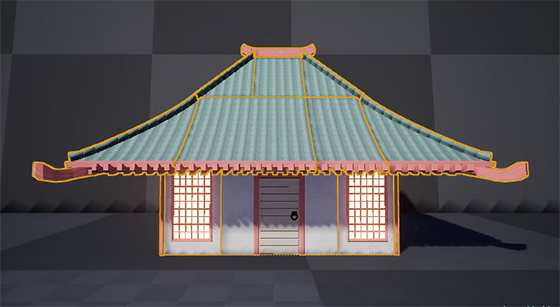
\includegraphics[width=\linewidth]{bilder/smallhousemodular}\newline
40 Module\\ \hline
\vspace{97pt}Großes \newline Gebäude&

\vspace{0.2pt}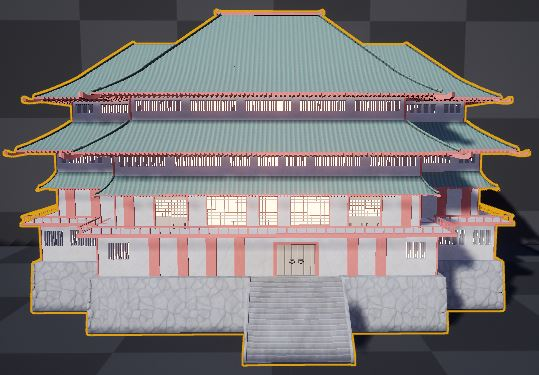
\includegraphics[width=\linewidth]{bilder/castleonepiece}\newline
155.000 Triangles, 8 Materialien &

\vspace{0.2pt}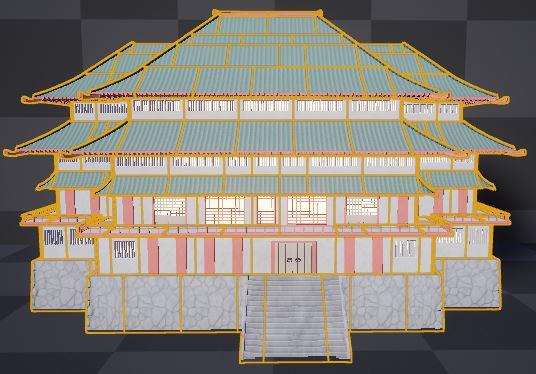
\includegraphics[width=\linewidth]{bilder/castlemodular}\newline
 342 Module\\ \hline
& 
\vspace{0.2pt}
Normale Ausführung &
\vspace{0.2pt}
Modulare Ausführung
\end{tabular}
 \caption{Aufbau und Eigenschaften der für die Performance-Test genutzten Gebäude.}
\end{table}
Für die Tests wurde ein leeres Level erstellt, in das eine Bodenebene und ein direktionales Licht eingefügt wurde. Mit Hilfe von Blueprints wurde das Level mit verschieden viel Gebäuden einer Art gefüllt. Nach Berechnung des Lichts wurden im Playmode verschiedene Werte gemessen. Der Test konnte auf der verwendeten Hardware mit 500 Gebäuden mit den großen Gebäuden nicht durchgeführt werden.
\begin{figure}[H]
\centering
  \makebox[\textwidth]{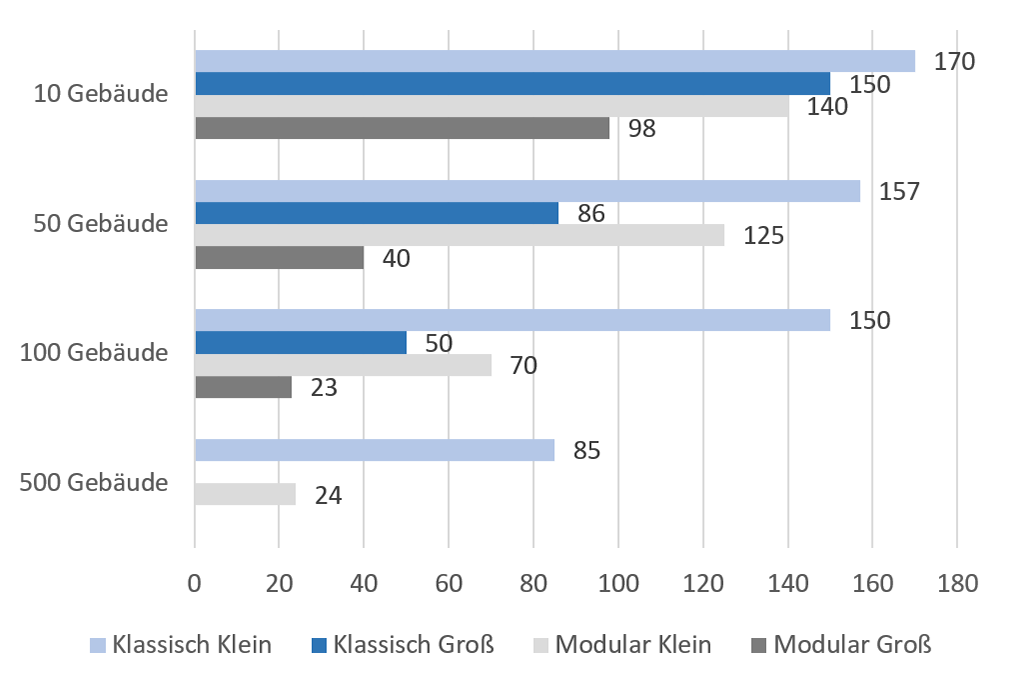
\includegraphics[width=\linewidth]{bilder/PerformancteTestFPS}}
  \caption{Übersicht der Bildfrequenzen aus den durchgeführten Tests.}
	\label{PerformancteTestFPS}
\end{figure}
\begin{figure}[H]
\centering
  \makebox[\textwidth]{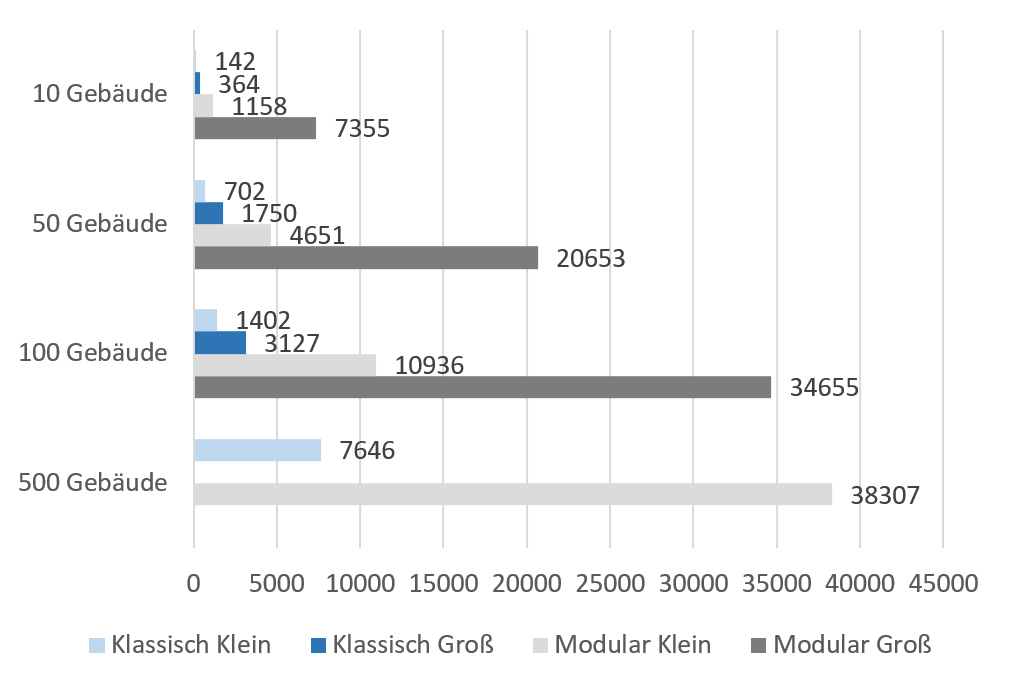
\includegraphics[width=\linewidth]{bilder/PerformancteTestDC}}
  \caption{Übersicht benötigter Draw Calls  aus den durchgeführten Tests.}
	\label{PerformancteTestDC}
\end{figure}
Die Diagramme zeigen, dass die Performance der nicht-modularen Gebäude deutlich besser ist. Die nötigen Draw Calls und die resultierende Last auf das System sind für die modularen Gebäude um ein Vielfaches höher als bei den nichtmodularen Gebäuden. Auch die Bildwiederholungsrate ist bei den klassischen Gebäuden bedeutend höher.
\par
Nach den Tests wurde versucht, die Performance der modularen Elemente zu verbessern. Das in Abschnitt \ref{Implementierung1} beschriebene \textit{Instancing} wird von der genutzten Version 4.21 von Unreal Engine nur teilweise automatisch angewendet. Die Modelle werden nur einmal in den Speicher geladen, aber jedes Modell erzeugt für sich und seine Materialien eigene Draw Calls.
\par
Mit Hilfe des Tools \enquote{AutoInstance}\footnote{\,Das Tool kann unter: \url{https://www.unrealengine.com/marketplace/en-US/slug/auto-instance} abgerufen werden.} aus dem Unreal Engine Marketplace wurde versucht das Instancing der Module zu verbessern.
\par
Das Tool konnte die Draw Calls drastisch verringern. Trotzdem konnte die Performance nicht verbessert werden, da durch das \textit{Instancing} an anderer Stelle neue Last entstand. Zudem wurde die Zuweisung der Materialien durch das Instanziieren der Module verändert und konnte nicht mehr angepasst werden.
\par
Die Instanziierung des Tools kann auch manuell durchgeführt werden, jedoch würde dies zu unverhältnismäßig viel Arbeit führen und müsste für jedes Level neu durchgeführt werden.
\par
In Unreal Engine können mehrere Objekte zu einem verbunden werden. Bei Tests dieser Funktion zeigte sich, dass bei der Verbindung von Modulen alle Material Slots erhalten bleiben. Dies hat aber zur Folge, dass wieder mehr Draw Calls erzeugt werden, als wenn das Gebäude in einem Stück in Unreal Engine importiert werden würde. Das große Gebäude aus dem Performance-Test hatte nach dem Verbinden in der Engine 737 zugewiesene Materialien anstelle von 8.
\par
Da die Performance-Unterschiede auch schon bei einer für das Spiel normalen bis geringen Anzahl von gleichzeitig sichtbaren Gebäude deutlich waren und es zu diesem Zeitpunkt keine Lösung gab, dies zu ändern, wurde davon abgesehen, das Kit in Unreal Engine zu nutzen.
\par
Die schon in Unreal Engine erstellten Gebäude wurden in Blender nachgebaut und in Unreal Engine importiert. Das Erstellen der Gebäude konnte in Blender mit einer höheren Geschwindigkeit durchgeführt werden als in Unreal Engine, da das 3D-Tool noch weitere Features für die Modellerstellung bietet.
\par
Der praktische Teil der Arbeit ist hier beendet, im Folgenden werden die Ergebnisse dieses Projektes zusammengefasst und ausgewertet.
\section{Ergebnisse}
In diesem Abschnitt wird zuerst darauf eingegangen, welche der zuvor erarbeiteten Methoden im Verlaufe des Projektes angewandt wurden und welchen Nutzen diese hatten. Im Anschluss wird das unter Anwendung der Methoden entstandene modulare Kit bewertet.
\begin{description}
\item[Raster]~\par
Ohne die Nutzung eines Rasters wäre das passgenaue Platzieren der Module so zeitaufwändig gewesen, dass es keinen Sinn ergeben würde ein modulares Kit zu nutzen.
\par
Auch bei der Erstellung der Module hat das Raster eine entscheidende Rolle gespielt. Ohne Anhaltspunkte, die durch das Raster gegeben waren, wäre es sehr schwer gewesen ein modulares System zu entwickeln, durch welches alle Teile miteinander verbunden werden können.
\par
Die von Burgess und Purkeypile erwähnte Methode, das Raster zu verlassen (siehe Abschnitt \ref{weitereT}) und an vorher platzierten Objekten auszurichten, wurde nicht genutzt. Dies hätte die Erstellung vieler neuer Module und Modifikationen  des Kits gefordert. Die Bauweise der nachzubildenden Gebäude bedient sich in der Regel nur rechten Winkeln, welche mit dem Kit dargestellt werden können. Es gab also auch keinen Grund diese Methode zu nutzen.
\item[Pivot Point]~\par
Nur durch die richtige Platzierung des Pivot Points konnte das volle Potenzial des Rasters genutzt werden. Der Pivot Point und seine Positionierung sind also eine genauso wichtige Komponente eines modularen Systems wie das Raster, welches ohne diesen nur bedingt genutzt werden kann. Für die Positionierung des Pivot Points wurden die Regeln\footnote{\,Eine Übersicht der Regeln kann in einem \textit{Gamasutra}-Artikel \parencite{Mader} von P. Mader unter dem Abschnitt \textit{Pivot Placement} gefunden werden.} von P. Mader genutzt.
\par
Sein Hinweis darauf den Pivot Point bei Objekten, die einen Kreis formen, in das Zentrum des Kreises zu setzen, wurde für dieses Objekt auch bei Eckmodulen angewandt. Dies beschleunigt die Neupositionierung und Ausrichtung dieser Elemente.
\item[Textur]~\par
Der Einsatz von kachelbaren Texturen war für das Kit unabdinglich. Darüber hinaus musste nicht viel beachtet werden außer, dass in der UV-Map die Ränder der Modelle mit den Rändern der Textur verbunden werden. Nur so war gewährleistet, dass es keine sichtbaren Kanten zwischen den Modulen gibt, die den Eindruck stören würden, dass das Gebäude aus einem Stück besteht.
\item[Planung und Tests]~\par
Ein weiterer wichtiger Aspekt des Projektes war das Planen und Testen. Auch wenn dies keine praktisch anwendbaren Methoden sind, wie die anderen hier aufgelisteten, sind sie nicht weniger wichtig.
\par
Ohne die vorherige Planung und diverse Tests, hätte die Entwicklung des Kits mehr Zeit in Anspruch genommen und hätte vermutlich keine so hohe Qualität erreicht.
\par
Mit der gewonnenen Erfahrung kann die Planungsphase bei dem nächsten Projekt schneller und besser durchgeführt werden. Viele der vorgenommenen Änderungen am Kit hätten durch mehr Praxiserfahrung schon in der ersten Planungsphase erkannt werden können, was den generellen Ablauf des Projektes beschleunigt hätte.
\par
Auf Tests und eventuelle Weiterentwicklungen des Kits sollte dennoch nicht verzichtet werden. Die in der Planungsphase erstellten Regeln sollten angepasst werden, wenn dadurch das Kit verbessert wird, auch wenn dadurch mehr Arbeit entsteht. Je nach Projekt wird das Kit an vielen Stellen und für lange Zeit genutzt und sollte daher so gut wie möglich ausgearbeitet sein.
\item[Varianten]~\par
Die Subkits bestehen aus allen nötigen Teilen, um verschiedene Gebäude zu bauen. Diese hätten alle ein sehr ähnliches Erscheinungsbild, wenn das Kit keine Varianten der Module enthalten würde. Bisher wurden nur von den Wand-, Balkon- und Holzbalkenelementen Varianten erstellt. Nur durch diese lassen sich schon viele individuell aussehende Gebäude erzeugen. Die Erzeugung weiterer Varianten nimmt nur wenig Zeit in Anspruch, da von einem Basis Modell aus gearbeitet werden kann, welches schon an die Regeln des Kits angepasst wurde.
\par
Das Nutzen von Varianten ist also ein effizienter Weg ein Kit zu ergänzen. Zusätzlich können, zumindest in Unreal Engine, Module einfach ausgetauscht werden. Hierfür muss, in dem Level, nur das gewünschte Modul ausgewählt werden und kann dann, durch ein Dropdown Menü, mit einem Anderen ersetzt werden. Durch eine passende Benennung stehen Varianten des Moduls in dem Dropdown Menü an der gleichen Stelle.
\item[Modularitätsstufen]~\par
Die Modularitätsstufe hat direkten Einfluss auf viele Aspekte des Kits und sollte dem Projekt entsprechend gewählt werden. Mit der Größe der Stufe verringert sich die Zeit, die benötigt wird ein fertiges Konstrukt zu erstellen. Die Abwechslung des Kits steht auch in Zusammenhang mit der eingesetzten Stufe und beeinflusst, wie viele Varianten der Module benötigt werden, um ein abwechslungsreiches Bild zu erzeugen. In diesem Projekt wurde eine mittlere bis kleine Stufe der Modularität gewählt. Folglich ist es möglich mit einer kleinen Auswahl an Modulen viele verschiedene Objekte zu erstellen. Würde ein Gebäude aus nur drei Modulen bestehen, müssten viel mehr Module erstellt werden, um die gleiche Abwechslung zu gewährleisten.
\par
Die Spielperformance wurde allerdings negativ durch die vielen genutzten Elemente beeinflusst. Dies konnte umgangen werden, indem die Gebäude in Blender vorgefertigt und im Anschluss als ein Objekt exportiert wurden.
\par
Die mögliche Diversität der gewählten Stufe geht hierdurch nicht verloren, da die Module auch in Blender genutzt werden können.
\item[Benennung]~\par
Eine gut konzipierte Benennung der Module ist wie von Burgess und Purkeypile angeführt ein sehr wichtiger Aspekt, um Arbeitsabläufe mit dem Kit zu beschleunigen und die Kommunikation zu verbessern. Wie zuvor beschrieben, muss darauf geachtet werden eine sinnvolle Bezeichnung der Module zu entwickeln, die leicht zu interpretieren und erlernen ist. Sind bei Tests Probleme mit Modulen aufgefallen, konnten diese leicht durch ihren Namen zugeordnet werden.
\item[Struktur]~\par
Zusammen mit der Benennung war das Einführen einer Ordnerstruktur sehr hilfreich, um den Prozess der Gebäudeerstellung in Unreal Engine zu beschleunigen. Auch wenn dies nur zu einem gewissen Grad getestet wurde. Des Weiteren konnte durch das Einteilen der Module in Subkits der Erstellungsprozess besser organisiert und die Übersicht in Unreal Engine dadurch deutlich verbessert werden.
\item[Vertex Farben]~\par
Das Einfärben von Vertices, um die Erscheinung der Texturen bzw. die des Models zu verändern, wurde nicht angewandt. Hierfür hätten weitere Module erstellt werden müssen. Da das Kit auch ohne diese Methode schon genug Abwechslung aufwies, wurde darauf verzichtet. Aufgrund des veränderten Arbeitsablaufes könnte dies, ohne großen Aufwand, für neue Gebäude genutzt werden, um mehr Abwechslung zu schaffen ohne neue Module zu entwickeln.
\end{description}
Die Bewertung der genutzten Methoden ist hier beendet. Im Folgenden werden die Eigenschaften des modularen Kits bewertet.
\begin{description}
\item[Visuelle Qualität]~\par
Gebäude, die mit dem neuen Kit erstellt wurden, erreichen das gleiche Level an Detail und Qualität, wie die schon bestehenden Assets und fügen sich sehr gut in den Spielstil ein.
\par
Test bezüglich der Kunstermüdung (siehe Abschnitt \ref{vqualitaet}) können aufgrund von fehlender Assets für ein gesamtes Level und der begrenzten Zeit nicht durchgeführt werden. Alle bisherigen Level wurden auf der Basis von neun Gebäuden erstellt. Mit dem modularen Set können weit mehr als neun verschiedene Gebäude erstellt werden. Das Nutzen des Kits sollte demnach keinen negativen Effekt auf das optische Erscheinungsbild des Levels haben.
\par
Durch weitere Varianten der Dachmodule könnte das Kit noch verbessert werden. Die Dächer aller Gebäude sehen gleich aus, auch wenn sie andere Formen haben.
\par
Durch das Zusammensetzen der Module in Blender kann jedes Modell, neben dem Kombinieren verschiedener Module auch ein individueller Look gegeben werden, indem das erstellte Gebäude durch Modifikationen der Meshes abgeändert wird. Hierdurch lässt sich die Qualität der Module weiter erhöhen, es wird aber auch weitere Arbeitszeit benötigt.	
\par
Die von Burgess und Purkeypile erwähnte Boxartigkeit von modularen Assets ist auch in diesem Set zu erkennen, dies ist jedoch zum Teil auf die Bauweise der Gebäude zurückzuführen, welche durch das Kit abgebildet werden sollten und fällt in diesem Fall nicht negativ auf.
\item[Nutzerfreundlichkeit]~\par
Die Handhabung sollte durch einen Level Designer geprüft werden, da die Modelle in Blender vorgefertigt werden müssen, wäre das Erstellen von Gebäuden in der Engine durch den Level Designer überflüssige Arbeit. Durch die durchgeführten Tests und die dadurch entstandenen Gebäude, wurde dennoch ein guter Eindruck der Handhabung vermittelt.
\par
Durch das genutzte Raster, die Platzierung des Pivot Points und die Benennung der Elemente fällt es sehr leicht Gebäude zu bauen. Gebäude von kleiner bis mittlerer Größe lassen sich schnell erstellen. Steigt die Größe des Gebäudes weiter an, erhöht sich die benötigte Zeit jedoch drastisch. Für größere Gebäude wäre es von Vorteil, wenn das Kit größere Elemente besitzen würde. Da aber hauptsächlich kleine bis mittlere Gebäude erstellt werden sollen, fällt dies nur gering negativ auf.
\par
Da in Blender die gleichen Methoden wie in Unreal Engine genutzt werden können und zusätzlich weitere Methoden zur Verfügung stehen, wurde die Nutzerfreundlichkeit in diesem Aspekt noch verbessert.
\item[Aufwand]~\par     
Das Erstellen der Assets hat viel Zeit gekostet, vor allem zu Beginn war es schwierig das Konzept der Modularität zu greifen und die Gebäude richtig in passende Module aufzuteilen, hierfür wurde die meiste Zeit der Planung aufgebracht.
\par
Nur für das eine Level wäre es vermutlich schneller gewesen einzelne Gebäude zu erstellen. Werden noch weitere Level in dem gleichen Setting entwickelt, kann der Arbeitsaufwand wohl ausgeglichen werden.
\par
Könnte das Kit, wie geplant, in Unreal Engine genutzt werden, hätte die benötigte Arbeitszeit, um Gebäude zu erstellen, besser auf das Team verteilt werden können. Das Erstellen und Anpassen der Gebäude aus den vorgefertigten Modulen wäre von den Level-Designern übernommen worden. So wäre es möglich gewesen, dass der 3D-Artist ohne Unterbrechungen an weiteren Assets für das Level arbeitet.
\par
Durch das Vorbauen der Modelle in Blender kann die Aussage von L. Durand  bezüglich der leichten und schnellen Anpassung der Gebäude auf das Gameplay nicht überprüft werden.
\item[Performance]~\par
Wie schon in Abschnitt \ref{implementierung2} beschrieben, war die Performance des modularen Kits, klassischen Assets in allen Aspekten weit unterlegen. Dies hatte zur Folge, dass das Kit nicht modular in Unreal Engine, sondern in Blender genutzt wird. In Unreal Engine werden normale Modelle genutzt, der Einfluss auf die Performance ist demnach genau so wie bei normal erstellten Assets.	
\end{description}